\documentclass{article}
\usepackage[utf8]{inputenc}
\usepackage[margin=0.4in]{geometry}


\title{Computer Networks HW 6}
\author{Shane Cincotta }
\date{May 13, 2020}

\usepackage{natbib}
\usepackage{graphicx}
\usepackage{amssymb}

\begin{document}

\maketitle

\section*{Chapter 5, Problem 3}
\begin{tabular}{ |l|l|l|l|l|l|l|l|}
  \hline
  Step & N' & D(t), p(t) & D(u), p(u) & D(v), p(v) & D(w), p(w) & D(y), p(y) & D(z), p(z)\\ \hline
  0 & x & inf & inf & 3,x & 6,x & 6,x & 8,x\\ \hline
  1 & xv & 7,v & 6,v & 3,x & 6,x & 6,x & 8,x\\ \hline
  2 & xvu & 7,v & 6,v & 3,x & 6,x & 6,x & 8,x\\ \hline
  3 & xvuw & 7,v & 6,v & 3,x & 6,x & 6,x & 8,x\\ \hline
  4 & xvuwy & 7,v & 6,v & 3,x & 6,x & 6,x & 8,x\\ \hline
  5 & xvuwyt & 7,v & 6,v & 3,x & 6,x & 6,x & 8,x\\ \hline
  6 & xvuwytz & 7,v & 6,v & 3,x & 6,x & 6,x & 8,x\\ \hline
\end{tabular}
\newline Thus the shortest paths from x along with their costs is: t:xvt = 7, u:xvu = 6, v:xv = 3, w:xw = 6, y:xy = 6 and z:xz = 8\\

\section*{Chapter 5, Problem 5}
\begin{tabular}{|l|l|l|l|l|l|}
\hline
& u & v & x & y & z \\ \hline
u & 0 & 1 & 4 & 2 & 6 \\ \hline
v & 1 & 0 & 3 & 3 & 5 \\ \hline
x & 4 & 3 & 0 & 3 & 2 \\ \hline
y & 2 & 3 & 3 & 0 & 5 \\ \hline
z & 6 & 5 & 2 & 5 & 0 \\ \hline
\end{tabular}

\section*{Chapter 5, Problem 7}
\subsection*{a}
\begin{tabular}{|l|l|l|l|}
\hline
Node & Description & Min Cost & Hop \\ \hline
X & Min cost from x to x & 0 & N/A \\ \hline
W & Min cost from x to w & 2 & - \\ \hline
Y & Min cost from x to y via w & 4 & W \\ \hline
U & Min cost from x to u & 7 & W \\ \hline
\end{tabular} 

\subsection*{b}
A change in c(x,y) $\leq$ 1 will result in x passing any changes onto its neighbors.\\
\newline When c(x,y) = $\delta \leq $ 1 then the hop done at y passes through the cose $\delta$ + 6 and node x will inform it's neighbors (y and w) of the new cost\\

\subsection*{c}
When c(x,y) -->5 is less than the min cost path from x to u (7), thus the cost is still at least 7.  The change in the cost of the link will not cause node x to inform it's neighbors of the new minimum cost path\\

\section*{Chapter 5, Problem 14}
\subsection*{a} Router 3c learns about prefix x from eBGP protocol\\
\subsection*{b} Router 3a learns about prefix x from iBGP protocol\\
\subsection*{c} Router 1c learns about x from from eBGP protocol\\
\subsection*{d} Router 1d learns about x from from iBGP protocol\\

\section*{Chapter 5, Problem 15}
\subsection*{a}
I will be equal to $I_1$ because the interface begins the least cost path at 1d towards the gateway router 1c\\

\subsection*{b}
I will be set to $I_2$ because router 1d learns about x from router 1b via AS2 through $I_2$ and learns x from router 1a via AS3 through $I_1$\\

\subsection*{c}
I will be set to $I_1$ because router 1d learns about x from router 1b via AS2 and reaches AS4 to get the value of x using the path $I_2$\\
\clearpage

\section*{Chapter 5, Problem 17}
\subsection*{a}
\begin{figure}[h!]
\centering
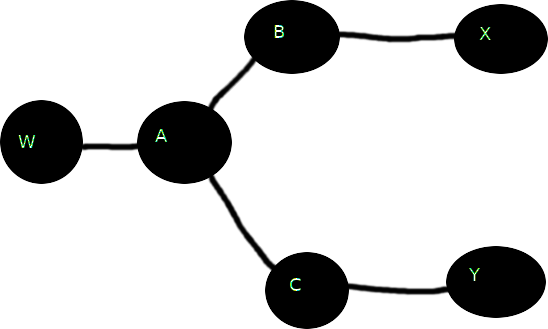
\includegraphics[scale=0.5]{Q17a.png}
\caption{W's view of the topology}
\end{figure}
The stub network W contains a path to the AS A.  The AS advertises the path of B and C to W, thus W can reach networks X and Y from A-B-X and A-C-Y (A doesn't know the path between B-C from W)\\

\subsection*{b}
\begin{figure}[h!]
\centering
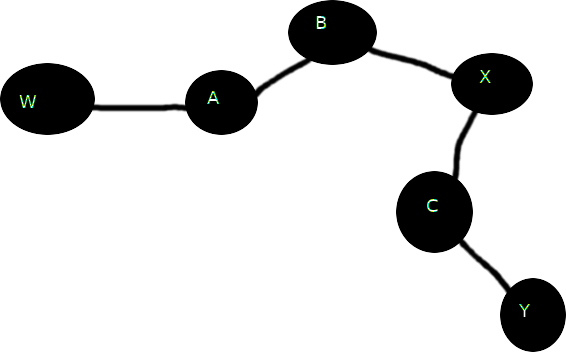
\includegraphics[scale=0.5]{Q17b.png}
\caption{X's view of the topology}
\end{figure}
X is a stubnetwork because it has two different providers, thus it receives from two prodvider networks.  For the first provider network, x receives from B and learns the path B-A-W.  For the second provider network, x receives from C and learns the path C-Y to reach Y (without knowing the link between A to C)\\

\section*{Chapter 5, Problem 20}
Yes BGP allows Z to ­implement this policy.  The BGP protocol allows Z to implement the policu by the way the BGP routes are handled.  That is, Y should advertise Xm X is unaware that Y has a path to Z and never forwards the traffic\\

\end{document}